%% abtex2-modelo-trabalho-academico.tex, v-1.9.7 laurocesar
%% Copyright 2012-2018 by abnTeX2 group at http://www.abntex.net.br/ 
%%
%% This work may be distributed and/or modified under the
%% conditions of the LaTeX Project Public License, either version 1.3
%% of this license or (at your option) any later version.
%% The latest version of this license is in
%%   http://www.latex-project.org/lppl.txt
%% and version 1.3 or later is part of all distributions of LaTeX
%% version 2005/12/01 or later.
%%
%% This work has the LPPL maintenance status `maintained'.
%% 
%% The Current Maintainer of this work is the abnTeX2 team, led
%% by Lauro César Araujo. Further information are available on 
%% http://www.abntex.net.br/
%%
%% This work consists of the files abntex2-modelo-trabalho-academico.tex,
%% abntex2-modelo-include-comandos and abntex2-modelo-references.bib
%%

% ------------------------------------------------------------------------
% ------------------------------------------------------------------------
% abnTeX2: Modelo de Trabalho Academico (tese de doutorado, dissertacao de
% mestrado e trabalhos monograficos em geral) em conformidade com 
% ABNT NBR 14724:2011: Informacao e documentacao - Trabalhos academicos -
% Apresentacao
% ------------------------------------------------------------------------
% ------------------------------------------------------------------------

\documentclass[
	% -- opções da classe memoir --
	12pt,				% tamanho da fonte
	openright,			% capítulos começam em pág ímpar (insere página vazia caso preciso)
	twoside,			% para impressão em recto e verso. Oposto a oneside
	a4paper,			% tamanho do papel. 
	% -- opções da classe abntex2 --
	%chapter=TITLE,		% títulos de capítulos convertidos em letras maiúsculas
	%section=TITLE,		% títulos de seções convertidos em letras maiúsculas
	%subsection=TITLE,	% títulos de subseções convertidos em letras maiúsculas
	%subsubsection=TITLE,% títulos de subsubseções convertidos em letras maiúsculas
	% -- opções do pacote babel --
	english,			% idioma adicional para hifenização
	french,				% idioma adicional para hifenização
	spanish,			% idioma adicional para hifenização
	brazil				% o último idioma é o principal do documento
	]{abntex2}

% ---
% Pacotes básicos 
% ---
\usepackage{lmodern}			% Usa a fonte Latin Modern			
\usepackage[T1]{fontenc}		% Selecao de codigos de fonte.
\usepackage[utf8]{inputenc}		% Codificacao do documento (conversão automática dos acentos)
\usepackage{indentfirst}		% Indenta o primeiro parágrafo de cada seção.
\usepackage{color}				% Controle das cores
\usepackage{graphicx}			% Inclusão de gráficos
\usepackage{microtype} 			% para melhorias de justificação
% ---
		
% ---
% Pacotes adicionais, usados apenas no âmbito do Modelo Canônico do abnteX2
% ---
\usepackage{lipsum}				% para geração de dummy text
% ---

% ---
% Pacotes de citações
% ---
\usepackage[brazilian,hyperpageref]{backref}	 % Paginas com as citações na bibl
\usepackage[alf]{abntex2cite}	% Citações padrão ABNT

% --- 
% CONFIGURAÇÕES DE PACOTES
% --- 

% ---
% Configurações do pacote backref
% Usado sem a opção hyperpageref de backref
\renewcommand{\backrefpagesname}{Citado na(s) página(s):~}
% Texto padrão antes do número das páginas
\renewcommand{\backref}{}
% Define os textos da citação
\renewcommand*{\backrefalt}[4]{
	\ifcase #1 %
		Nenhuma citação no texto.%
	\or
		Citado na página #2.%
	\else
		Citado #1 vezes nas páginas #2.%
	\fi}%
% ---

% ---
% Informações de dados para CAPA e FOLHA DE ROSTO
% ---
\titulo{Estudo de Oscilações de Estados em Autômatos Celulares com Inércia}
\autor{Ly Sandro Amorim de Campos Salles}
\local{Curitiba}
\data{2019}
\orientador{Marlus Koehler}
\coorientador{}
\instituicao{%
  Universidade Federal do Paraná -- UFPR
  \par
  Departamento de Física}
\tipotrabalho{Trabalho de Conclusão de Curso}
% O preambulo deve conter o tipo do trabalho, o objetivo, 
% o nome da instituição e a área de concentração 
\preambulo{Trabalho de Conclusão de Curso apresentado à banca examinadora como requisito para a aprovação na disciplica TCC-B (CF1811) do curso de Licenciatura em Física da Universidade Federal do Paraná.}
% ---


% ---
% Configurações de aparência do PDF final

% alterando o aspecto da cor azul
\definecolor{blue}{RGB}{0,0,0}

% informações do PDF
\makeatletter
\hypersetup{
     	%pagebackref=true,
		pdftitle={\@title}, 
		pdfauthor={\@author},
    	pdfsubject={\imprimirpreambulo},
	    pdfcreator={LaTeX with abnTeX2},
		pdfkeywords={abnt}{latex}{abntex}{abntex2}{trabalho acadêmico}, 
		colorlinks=true,       		% false: boxed links; true: colored links
    	linkcolor=blue,          	% color of internal links
    	citecolor=blue,        		% color of links to bibliography
    	filecolor=magenta,      		% color of file links
		urlcolor=blue,
		bookmarksdepth=4
}
\makeatother
% --- 

% ---
% Posiciona figuras e tabelas no topo da página quando adicionadas sozinhas
% em um página em branco. Ver https://github.com/abntex/abntex2/issues/170
\makeatletter
\setlength{\@fptop}{5pt} % Set distance from top of page to first float
\makeatother
% ---

% ---
% Possibilita criação de Quadros e Lista de quadros.
% Ver https://github.com/abntex/abntex2/issues/176
%
\newcommand{\quadroname}{Quadro}
\newcommand{\listofquadrosname}{Lista de quadros}

\newfloat[chapter]{quadro}{loq}{\quadroname}
\newlistof{listofquadros}{loq}{\listofquadrosname}
\newlistentry{quadro}{loq}{0}

% configurações para atender às regras da ABNT
\setfloatadjustment{quadro}{\centering}
\counterwithout{quadro}{chapter}
\renewcommand{\cftquadroname}{\quadroname\space} 
\renewcommand*{\cftquadroaftersnum}{\hfill--\hfill}

\setfloatlocations{quadro}{hbtp} % Ver https://github.com/abntex/abntex2/issues/176
% ---

% --- 
% Espaçamentos entre linhas e parágrafos 
% --- 

% O tamanho do parágrafo é dado por:
\setlength{\parindent}{1.3cm}

% Controle do espaçamento entre um parágrafo e outro:
\setlength{\parskip}{0.2cm}  % tente também \onelineskip

% ---
% compila o indice
% ---
\makeindex
% ---

% ----
% Início do documento
% ----
\begin{document}

% Seleciona o idioma do documento (conforme pacotes do babel)
%\selectlanguage{english}
\selectlanguage{brazil}

% Retira espaço extra obsoleto entre as frases.
\frenchspacing 

% ----------------------------------------------------------
% ELEMENTOS PRÉ-TEXTUAIS
% ----------------------------------------------------------
% \pretextual

% ---
% Capa
% ---
\imprimircapa
% ---

% ---
% Folha de rosto
% (o * indica que haverá a ficha bibliográfica)
% ---
\imprimirfolhaderosto*
% ---

% ---
% Inserir a ficha bibliografica
% ---

% Isto é um exemplo de Ficha Catalográfica, ou ``Dados internacionais de
% catalogação-na-publicação''. Você pode utilizar este modelo como referência. 
% Porém, provavelmente a biblioteca da sua universidade lhe fornecerá um PDF
% com a ficha catalográfica definitiva após a defesa do trabalho. Quando estiver
% com o documento, salve-o como PDF no diretório do seu projeto e substitua todo
% o conteúdo de implementação deste arquivo pelo comando abaixo:
%
% \begin{fichacatalografica}
%     \includepdf{fig_ficha_catalografica.pdf}
% \end{fichacatalografica}

\begin{fichacatalografica}
	\sffamily
	\vspace*{\fill}					% Posição vertical
	\begin{center}					% Minipage Centralizado
	\fbox{\begin{minipage}[c][8cm]{13.5cm}		% Largura
	\small
	\imprimirautor
	%Sobrenome, Nome do autor
	
	\hspace{0.5cm} \imprimirtitulo  / \imprimirautor. --
	\imprimirlocal, \imprimirdata-
	
	\hspace{0.5cm} \thelastpage p. : il. (algumas color.) ; 30 cm.\\
	
	\hspace{0.5cm} \imprimirorientadorRotulo~\imprimirorientador\\
	
	\hspace{0.5cm}
	\parbox[t]{\textwidth}{\imprimirtipotrabalho~--~\imprimirinstituicao,
	\imprimirdata.}\\
	
	\hspace{0.5cm}
		1. Palavra-chave1.
		2. Palavra-chave2.
		2. Palavra-chave3.
		I. Marlus Koehler.
		II. Universidade Federal do Paraná.
		III. Departamento de Física.
		IV. Estudo de Oscilações de Estados em Autômatos Celulares com Inércia.
	\end{minipage}}
	\end{center}
\end{fichacatalografica}
% ---

% ---
% Inserir errata
% ---
%\begin{errata}
%Elemento opcional da \citeonline[4.2.1.2]{NBR14724:2011}. Exemplo:
%
%\vspace{\onelineskip}
%
%FERRIGNO, C. R. A. \textbf{Tratamento de neoplasias ósseas apendiculares com
%reimplantação de enxerto ósseo autólogo autoclavado associado ao plasma
%rico em plaquetas}: estudo crítico na cirurgia de preservação de membro em
%cães. 2011. 128 f. Tese (Livre-Docência) - Faculdade de Medicina Veterinária e
%Zootecnia, Universidade de São Paulo, São Paulo, 2011.
%
%\begin{table}[htb]
%\center
%\footnotesize
%\begin{tabular}{|p{1.4cm}|p{1cm}|p{3cm}|p{3cm}|}
%  \hline
%   \textbf{Folha} & \textbf{Linha}  & \textbf{Onde se lê}  & \textbf{Leia-se}  \\
%    \hline
%    1 & 10 & auto-conclavo & autoconclavo\\
%   \hline
%\end{tabular}
%\end{table}
%
%\end{errata}
% ---

% ---
% Inserir folha de aprovação
% ---

% Isto é um exemplo de Folha de aprovação, elemento obrigatório da NBR
% 14724/2011 (seção 4.2.1.3). Você pode utilizar este modelo até a aprovação
% do trabalho. Após isso, substitua todo o conteúdo deste arquivo por uma
% imagem da página assinada pela banca com o comando abaixo:
%
% \begin{folhadeaprovacao}
% \includepdf{folhadeaprovacao_final.pdf}
% \end{folhadeaprovacao}
%
%\begin{folhadeaprovacao}

%  \begin{center}
%    {\ABNTEXchapterfont\large\imprimirautor}

%    \vspace*{\fill}\vspace*{\fill}
%    \begin{center}
%      \ABNTEXchapterfont\bfseries\Large\imprimirtitulo
%    \end{center}
%    \vspace*{\fill}
%    
%    \hspace{.45\textwidth}
%    \begin{minipage}{.5\textwidth}
%        \imprimirpreambulo
%    \end{minipage}%
%    \vspace*{\fill}
%   \end{center}
%        
%   Trabalho aprovado. \imprimirlocal,  de novembro de 2012:

%   %\assinatura{\textbf{\imprimirorientador} \\ Orientador} 
%   \assinatura{\textbf{Professor} \\ Convidado 1}
%   \assinatura{\textbf{Professor} \\ Convidado 2}
%   \assinatura{\textbf{Professor} \\ Convidado 3}
%   %\assinatura{\textbf{Professor} \\ Convidado 4}
%      
%   \begin{center}
%    \vspace*{0.5cm}
%    {\large\imprimirlocal}
%    \par
%    {\large\imprimirdata}
%    \vspace*{1cm}
%  \end{center}
%  
%\end{folhadeaprovacao}
% ---

% ---
% Dedicatória
% ---
%\begin{dedicatoria}
%   \vspace*{\fill}
%   \centering
%   \noindent
%   \textit{ Este trabalho é dedicado às crianças adultas que,\\
%   quando pequenas, sonharam em se tornar cientistas.} \vspace*{\fill}
%\end{dedicatoria}
% ---

% ---
% Agradecimentos
% ---
\begin{agradecimentos}
Agradeço ao meu Orientador Marlus Koehler pela liberdade e pela confiança no meu trabalho.

\end{agradecimentos}
% ---

% ---
% Epígrafe
% ---
\begin{epigrafe}
    \vspace*{\fill}
	\begin{flushright}
		\textit{``Texto\\
		Tente outra vez\\
		''\\
		(Livro das Virtudes para Crianças)}
	\end{flushright}
\end{epigrafe}
% ---

% ---
% RESUMOS
% ---

% resumo em português
\setlength{\absparsep}{18pt} % ajusta o espaçamento dos parágrafos do resumo
\begin{resumo}
  Utilizando um autômato celular bidimensional desenvolvido por Dietrich Stauffer e Gérard Weisbuch em 2002 para simulações de agentes em estado de compra ou venda em um sistema, determinamos a intensidade com que esses agentes tendem a tomar decisões em conjunto, denominada afinidade. Isso foi feito considerando vizinhanças de Moore e Von Neumann. Desenvolvemos duas interpretações para a variável que determina a velocidade do sistema: liquidez, e volatilidade. Essas simulações foram feitas para números diferentes de agentes, variando de 2500 a 250000. Descobrimos, nessa análise positiva, que a afinidade é uma função sigmóide da liquidez, variando com o número de agentes. Com base nesses dados percebemos que, para sistemas com alta liquidez, como o mercado de alimentos na vida real, a tendência de aglomeração de agentes é alta, o que pode explicar a existência das Centrais de Abastecimento CEASA. Analogamente, quando a liquidez é baixa, como no caso das negociações envolvendo itens de colecionador e figurinhas de copa do mundo, a tendência de aglomeração é menor, fazendo com que existam mais aglomerados esparsamente distribuídos, como grupos de troca de figurinhas em várias praças de uma mesma cidade. Com a análise de volatilidade foi percebido um comportamento semelhante ao de mercados financeiros, sendo a oscilação do preço do produto defasada em relação à oscilação do número de compradores. Aproveitando a forma com que computadores geram números aleatórios também foi possível verificar se os autômatos celulares estudados apresentavam comportamento caótico. Colateralmente foi desenvolvido um algoritmo de contagem de aglomerados para autômatos celulares em duas dimensões que se mostrou mais eficiente do que os utilizados atualmente ao considerar um algoritmo semelhante ao processo de contaminação celular.

 \textbf{Palavras-chave}: Autômato celular. Aglomeração. Análise positiva. Liquidez. Volatilidade. Estocasticidade. Modelagem. Econofísica. Microeconomia. Caos.
\end{resumo}

% resumo em inglês
\begin{resumo}[Abstract]
 \begin{otherlanguage*}{english}
   This is the english abstract.

   \vspace{\onelineskip}
 
   \noindent 
   \textbf{Keywords}: latex. abntex. text editoration.
 \end{otherlanguage*}
\end{resumo}
% ---

% ---
% inserir lista de ilustrações
% ---
\pdfbookmark[0]{\listfigurename}{lof}
\listoffigures*
\cleardoublepage
% ---

% ---
% inserir lista de quadros
% ---
\pdfbookmark[0]{\listofquadrosname}{loq}
\listofquadros*
\cleardoublepage
% ---

% ---
% inserir lista de tabelas
% ---
\pdfbookmark[0]{\listtablename}{lot}
\listoftables*
\cleardoublepage
% ---

% ---
% inserir lista de abreviaturas e siglas
% ---
\begin{siglas}
  \item[UFPR] Universidade Federal do Paraná
  \item[ICA ou INCA] Inhomogenous Cellular Automata
\end{siglas}
% ---

% ---
% inserir lista de símbolos
% ---
\begin{simbolos}
  \item[$ \forall $] Para todo
  \item[$ \Rightarrow $] Implica
  \item[$ \Leftrightarrow $] Se, e somente se
  \item[$ \in $] Pertence
\end{simbolos}
% ---

% ---
% inserir o sumario
% ---
\pdfbookmark[0]{\contentsname}{toc}
\tableofcontents*
\cleardoublepage
% ---



% ----------------------------------------------------------
% ELEMENTOS TEXTUAIS
% ----------------------------------------------------------
\textual

% ----------------------------------------------------------
% Introdução (exemplo de capítulo sem numeração, mas presente no Sumário)
% ----------------------------------------------------------
\chapter{Introdução}
% ----------------------------------------------------------

Autômatos são objetos que operam a si mesmos. Essa definição, disponível na Encyclopaedia Britannica (Referências \cite{britannica1} e \cite{britannica2}), traz a possibilidade de objetos de uso cotidiano, como o computador e o celular, se encaixarem na categoria de autômatos. Porém, a existência de desses objetos não é nova, existindo autômatos desde a Grécia antiga na figura de um modelo de madeira de um pombo construído por Archytas de Tarentum. Utilizações contemporâneas de autômatos incluem as redes neurais e as inteligências artificiais. Também existem outros tipos famosos de autômatos, como os autômatos celulares.

Os autômatos celulares são, segundo a Encyclopaedia Britannica (referência \cite{britannica3}), simples modelos espacialmente distribuídos capazes de simular processos do mundo real. Eles foram inventados por John von Neumann e Stanislaw Ulam no Laboratório Nacional de Los Alamos em 1940 e ficaram famosos através do ``Game of Life'', inventado por John Conway em 1970, que simula a dinâmica de vida, morte e população.

Em 2003, Dietrich Stauffer (Referência \cite{stauffer}) publicou um artigo no qual ele descreveu um autômato celular não-homogêneo (chamado por ele de InCA ou Inhomogeneous Cellullar Automata) no qual a atualização das células ocorria de forma aleatória e cada célula tinha uma espécie de resistência interna a mudar de estado. Formalmente, em uma matriz, cada célula do autômato de Stauffer guarda dois números: o próprio estado e o próprio limiar. O limiar é definido como sendo o menor valor da soma dos estados das células vizinhas necessário para que a célula fique no estado $+1$ caso ela seja atualizada. Caso a célula seja atualizada mas ela não tenha um número de vizinhos no estado $+1$ suficiente para ficar no estado $+1$, a célula fica no estado $-1$ e seu limiar diminui por um número aleatório entre $0$ e $q$, onde $q$ é o ajuste máximo de limiar, definido antes do início da simulação. Caso a célula fique no estado $+1$ ao ser atualizada, o seu limiar aumenta por um número aleatório entre $0$ e $q$.

Em seu artigo ``Adjustment and social choice'' (Referência \cite{stauffer}), Stauffer explorou o comportamento das oscilações do estado médio e do limiar médio da matriz em função do tempo de simulação. Nisso ele percebeu que, quanto maior o valor do ajuste máximo de limiar $q$, maior é a frequência dessas oscilações em função do tempo. Stauffer utilizou os resultados obtidos para propor previsões e modelos para mercados financeiros.

Já em 2014, Klaus Kramer (Referência \cite{klaus}) desenvolveu estudos sobre autômatos celulares envolvendo três estados e focou na formação de aglomerados. Dos três estados, dois ($+1$ e $-1$) eram competitivamente ativos pois competiam entre si e um -- o estado $0$ -- era competitivamente passivo pois não competia com os outros estados. A regra de atualização utilizada foi semelhante à de Stauffer, com a diferença de o limiar de cada célula permanecer constante ao longo de toda a simulação. Além disso, nesse modelo as células com pelo menos uma célula vizinha no estado $0$ têm chances aleatórias de mudar para o estado $0$. Por fim, Kramer relacionou os estudos realizados com áreas de transição entre biomas diferentes.

Tendo como base esses autores, o objetivo deste trabalho foi explorar a dinâmica oscilatória do autômato celular de Stauffer, juntando a ele a ideia de estudar aglomerados empreendida por Kramer, a fim de buscar padrões que possam ser associados a fenômenos naturais.

\section*{Objetivos}

\subsection*{Objetivo geral:}

\subsection*{Objetivos específicos:}
\begin{enumerate}
  \item O1
\end{enumerate}

% ----------------------------------------------------------
% PARTE
% ----------------------------------------------------------
\part{Preparação da pesquisa}
% ----------------------------------------------------------

\section*{Metodologia}

\subsection*{Estudos iniciais}

O primeiro passo para este estudo foi conhecer a produção científica sobre autômatos celulares na área da Física. Para isso foram lidos alguns artigos, incluindo:
\begin{enumerate}
    \item Rodrigo de Lazzari: “Estudo De Um Autômato Celular Para Modelar Ciclos De Expansão E Contração (“Boom E Burst”)” (Referência \cite{lazzari});
    \item Klaus Kramer: “Dinâmica de padrões em autômatos celulares com inércia” (Referência \cite{klaus});
    \item Gérard Weisbuch, Dietrich Stauffer: “Adjustment and social choice” (Referência \cite{stauffer});
\end{enumerate}
Também foram verificadas implementações de autômatos celulares  com o software de simulações científicas Netlogo. Ainda foi feita a leitura de alguns artigos sobre estatística e correlação para auxiliar na interpretação dos dados gerados pelas simulações. Adicionalmente, com o objetivo de obter conhecimento para criar implementações de autômatos celulares na linguagem de programação C, foram  lidos vários capítulos do livro “C programming: A modern approach, 2nd Edition” do autor K.N. King (Referência \cite{king}).
    
\subsection*{Desenvolvimentos}

O primeiro desenvolvimento foi a percepção de características recorrentes nos autômatos celulares observados nos Estudos Iniciais.
A seguinte lista de características de autômatos celulares foi produzida com base nos artigos e software explorados:\\
\underline{Número de estados:} Quantos estados cada célula pode assumir.\\
\underline{Competitividade ou simbiose entre estados:} se a existência de um estado favorece ou inibe, nas proximidades, a existência de estados diferentes.\\
\underline{Vizinhança interna:} a região que é considerada interna a cada célula.\\
\underline{Vizinhança externa:} a região que é considerada externa a cada célula, apesar de ser próxima o suficiente para afetar diretamente o comportamento da célula.\\
\underline{Determinismo ou estocasticidade:} se a atualização das células ocorre de maneira previsível ou aleatoriamente.\\
\underline{Topologia do espaço:} como as bordas ou células estão conectadas.\\
\underline{Geometria do espaço:} formato das células e organização delas no espaço, caso aplicável.\\
\underline{Regras para atualização das células:} regras que determinam qual será o estado da célula no próximo passo ou ciclo da simulação.\\
\underline{Superposição de estados:} se é possível que cada célula tenha mais de um estado ao mesmo tempo.\\
\underline{Propriedades intrínsecas a cada célula:} características únicas a cada célula, além do estado.

O autômatos celular não-homogêneo (InCA) de Stauffer foi modelado utilizando as características acima, resultando na descrição abaixo:\\
\underline{Número de estados:} Dois estados, -1 e 1.\\
\underline{Competitividade ou simbiose entre estados:} competitividade.\\
\underline{Topologia do espaço:} quadrada de tamanho $L\times L$, onde $L$ é a \textit{largura da matriz} em unidades de números de células, com bordas fechadas. Células conectadas verticalmente e horizontalmente por vizinhança mais próxima, mas não diagonalmente..\\
\underline{Geometria do espaço:} malha quadrada.\\
\underline{Vizinhança interna:} quadrada de raio 0 (somente a própria célula).\\
\underline{Vizinhança externa:} Cruz com eixos paralelos à malha da geometria do espaço. Raio 1. Formato de +. Vizinhança mais próxima. Células nas posições Norte, Sul, Leste e Oeste em relação à célula considerada.\\
\underline{Determinismo ou estocasticidade:} estocasticidade porque, em cada passo, uma célula escolhida aleatoriamente é atualizada com um parâmetro de valor aleatório.\\
\underline{Propriedades intrínsecas a cada célula:} cada célula $\mathbf{x}$ tem um valor intrínseco $\lambda_\mathbf{x}$, chamado \textit{limiar}, que determina qual a menor soma dos estados das células da vizinhança externa necessária para que a célula fique no estado +1 caso ela seja atualizada.\\
\underline{Regras para atualização das células:}  dada uma célula $\mathbf{x}$, caso ela seja atualizada, o limiar $\lambda_\mathbf{x}$ aumenta caso a célula fique +1 e diminui caso a célula fique -1. O valor $|\Delta\lambda_\mathbf{x}|$ é gerado aleatoriamente e está entre $0$ e $q$, onde $q$ é o \textit{ajuste máximo de limiar}.\\
\underline{Superposição de estados:} Não, somente um estado por célula.\\


Em seguida, esse modelo de autômatos celular foi implementado na linguagem C. Para cada simulação, a matriz foi inicializada com valores $-1$ ou $+1$ dispostos aleatoriamente mas de modo que a diferença entre o número de células positivas e o número de células negativas fosse menor que 1\% do número total de células na matriz. Para todas as células o limiar foi iniciado em $\lambda_\mathbf{x} = 0$. A Figura \ref{fig:matrizL100Ciclo0} exibe a matriz estado inicial gerada em uma execução do InCA implementado.

\begin{figure}
    \centering
    %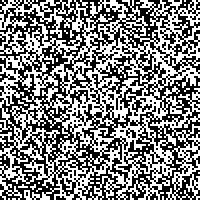
\includegraphics[width=0.7\linewidth]{matrizL100Ciclo0.png}
    \caption{Representação gráfica da matriz de estados iniciais de uma simulação com $L=100$. Células pretas representam o estado $-1$ e células brancas representam o estado $+1$. A matriz de estados iniciais é gerada de forma a manter o número de células positivas próximo ao número de células negativas.}
    \label{fig:matrizL100Ciclo0}
\end{figure}

O grande diferencial desta implementação do InCA, em relação ao estudo de Stauffer, foi a utilização de um algoritmo de contagem de aglomerados de células com o mesmo estado. Esse algoritmo, ilustrado na Figura \ref{fig:contamination}, encontra todas as células em um mesmo aglomerado através de ``contaminações'' sucessivas de células com o mesmo estado que são vizinhas entre si.

\begin{figure}
    \centering
    %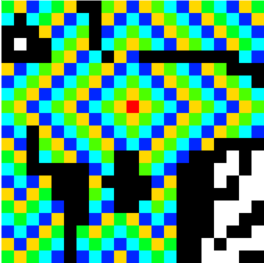
\includegraphics[width=.7\linewidth]{contamination.png}
    \caption{Algoritmo de contagem de aglomerados por contaminação de células vizinhas com o mesmo estado. Cada aglomerado é contaminado a partir de uma primeira célula até que não existam mais células a serem contaminadas. Na figura, a primeira célula é a central (em vermelho). Em seguida, as quatro células adjacentes a essa célula são contaminadas. No passo seguinte as oito células adjacentes a essas quatro células são contaminadas. O processo é repetido até que não existam mais células a serem contaminadas.}
    \label{fig:contamination}
\end{figure}

A implementação do InCA foi planejada para imprimir várias informações sobre a situação da matriz: Ciclo, Estado Médio da matriz, Limiar Médio da matriz, Número de Aglomerados e Índice de células Positivas que Pertencem a Algum Aglomerado (número total de células positivas em algum aglomerado dividido pelo número total de células na matriz). Um \textit{Ciclo} foi definido como sendo igual a $L\times L$ atualizações aleatórias de células na matriz, já que esse seria o número de atualizações de células caso o sistema fosse determinístico.

\subsection*{Metodologias de análise}

As análises foram feitas graficamente com os dados de estado médio, limiar médio, número de aglomerados e índice de células pertencentes a aglomerados em função do ciclo da simulação. Nesses gráficos foram buscados padrões recorrentes, como retas, parábolas ou elipses. Para isso foram feitas 288 simulações, variando a largura da matriz pelos valores 100, 250,
500,
750,
1000,
1250,
1500,
1750 e
2000, e o ajuste máximo de limiar entre os valores 0.5,
0.75,
1,
1.5,
2,
3,
4,
5,
6,
7,
8,
9,
10,
11,
12,
13,
14,
15,
16,
17,
18,
19,
20,
25,
30,
35,
40,
45,
50,
100,
150,
200 e
500.

\section*{Resultados Parciais Alcançados}

O primeiro estudo foi realizado quanto ao efeito da topologia no comportamento do valor médio e do limiar médio em função do ciclo. Foi observado que topologias com bordas conectadas apresentam gráficos mais suaves em relação a topologias com bordas fechadas. %Isso está ilustrado nas Figuras \ref{fig:topocaixa} e \ref{fig:topotorus}.

%\begin{figure}
%    \centering
%    \includegraphics[width=.9\linewidth]{topocaixa%.png}
%    \caption{Topologia de caixa}
%    \label{fig:topocaixa}
%\end{figure}
%
%\begin{figure}
%    \centering
%    \includegraphics[width=.9\linewidth]{topotorus%.png}
%    \caption{Topologia de Torus}
%    \label{fig:topotorus}
%\end{figure}

O segundo estudo foi feito quanto ao número de aglomerados e índice de células pertencentes a aglomerados. Também foi explorada a relação entre estado médio e número de aglomerados. Foi observado que o índice de células em aglomerados aumenta quando o estado médio fica positivo, como ilustrado na Figura \ref{fig:dataL2000Q100CellInClusterAvgStateVsCycle}. 
\begin{figure}[h]
    \centering
    %\includegraphics[width=.9\linewidth]{dataL2000Q100CellInClusterAvgStateVsCycle.png}
    \caption{Demonstração da correlação entre o índice de células positivas que pertencem a algum aglomerado e o estado médio do sistema. Quando o estado médio fica mais positivo (existem mais células positivas), o índice de células positivas em aglomerados aumenta proporcionalmente. Analogamente, se o estado médio diminui, o índice de células positivas em aglomerados também diminui.}
    \label{fig:dataL2000Q100CellInClusterAvgStateVsCycle}
\end{figure}
Isso demonstra que esses dois valores estão correlacionados, implicando que as células tendem a estarem aglomeradas. 

Quanto à relação entre o número de aglomerados em função do estado médio, foi constatado que estes tendem a estar relacionados linearmente como na Figura \ref{fig:dataL1750Q100ClustersVsAvgState}. 
\begin{figure}[h]
    \centering
    %\includegraphics[width=.9\linewidth]{dataL1750Q100ClustersVsAvgState.png}
    \caption{Exemplo da tendência de o número de aglomerados tender a ser linearmente dependente ao estado médio. Este gráfico contém 300 pontos de dados obtidos numa simulação com ajuste máximo de limiar igual a $1.00$ e largura de matriz igual a $1750$. Esse padrão foi observado em todas as outras medições realizadas.}
    \label{fig:dataL1750Q100ClustersVsAvgState}
\end{figure}
Uma análise dos coeficientes angulares das retas que melhor aproximam esses dados (através do Método dos Mínimos Quadrados) para várias larguras de matrizes e vários valores de ajuste máximo de limiar revelou que os gráficos desses coeficientes angulares em função de $q$ apresentam um ``vale'' semelhante ao do potencial de Lennard-Jones, como exibido na Figura \ref{fig:DadosSlopeL1000}.
\begin{figure}
    \centering
    %\includegraphics[width=.9\linewidth]{DadosSlopeL1000.png}
    \caption{Exemplo da curva  em função do ajuste máximo de limiar $q$ encontrada para a maioria dos gráficos das inclinações do número de aglomerados \textit{versus} estado médio. Inicialmente foi conjecturada uma semelhança como potencial de Lennard-Jones.}
    \label{fig:DadosSlopeL1000}
\end{figure}
A presença desse ``poço'' em todas as simulações realizadas incentivou a definição da afinidade em função do ajuste máximo de limiar.

\textbf{Definição:} No InCA, seja $I_{q,L}$ a inclinação da reta que melhor aproxima os dados obtidos em uma simulação com ajuste máximo de limiar igual a $q$ e largura de matriz $L$. Seja $Imin_L$ a menor inclinação para um dado $L$. Definimos a \textit{afinidade em função de $q$ e $L$} como sendo $A_{q,L}=-I_{q,L}/Imin_L$.

Contudo, ao analisar a afinidade para várias larguras $L$ diferentes, foi verificado que a Afinidade independe da largura da matriz, como está exibido na Figura \ref{fig:afinidadesQ0a200L750a2000}.
\begin{figure}
    \centering
    %\includegraphics[width=.9\linewidth]{afinidadesQ0a200L750a2000.png}
    \caption{Demonstração da independência da afinidade em relação à largura $L$ da matriz utilizada nas simulações. A sobreposição das seis curvas é aproximadamente absoluta até $q\approx 30$, divergindo levemente entre $q\approx 50$ e $q\approx 200$ devido à natureza estocástica da simulação.}
    \label{fig:afinidadesQ0a200L750a2000}
\end{figure}
Esse fato, corroborado pelo mapa da Figura \ref{fig:afinidadesHeatmap},
incentiva a seguinte definição:

\textbf{Definição:} A \textit{afinidade em função de $q$} é dada pelo valor médio da \textit{afinidade em função de $q$ e $L$} através de várias medições para vários valores de $L$.

Com base nessa definição, foi encontrado o gráfico da afinidade através das simulações realizadas. Esse gráfico está exibido na Figura \ref{fig:afinidadeMedia}.

Também foram buscados padrões de caos e atratores na dinâmica não-linear das simulações realizadas, sendo encontrados vários gráficos com comportamentos interessantes, como o da Figura \ref{fig:dataL1000Q75ClustersVsAvgThres}. Contudo, ainda não foi verificado se existe caos nesses sistemas.

Por fim foram feitas simulações considerando matrizes em três dimensões, nas quais foi possível constatar comportamentos análogos aos observados no caso de duas dimensões, como a relação entre estado médio e limiar médio em função do ciclo de simulação, além da linearidade do número de aglomerados em função do estado médio. Trabalhos nessas simulações foram descontinuados devido a incertezas sobre a precisão do código utilizado.


% ----------------------------------------------------------
% Finaliza a parte no bookmark do PDF
% para que se inicie o bookmark na raiz
% e adiciona espaço de parte no Sumário
% ----------------------------------------------------------
\phantompart

% ---
% Conclusão
% ---
\chapter{Conclusão}
% ---

Com os trabalhos desenvolvidos neste semestre foi possível desenvolver habilidades de análise e reprodução de autômatos celulares (em especial o \textit{Inhomogenous Cellular Automata} de Stauffer). A grande surpresa do estudo aconteceu nos recorrentes padrões lineares no caso dos gráficos do número de aglomerados em função do estado médio, sendo ainda mais surpreendente a independência da afinidade em relação à largura da matriz utilizada. A existência de discos como atratores de vários dos gráficos de número número de aglomeros em função do limiar médio também foi inesperada. Dos estudos relacionados à simulações em três dimensões, foi fortalecida a necessidade de códigos de programação bem organizados, a fim de evitar incertezas sobre a validade dos resultados.

Os próximos passos incluem estudar o motivo da existência do máximo no gráfico da afinidade média (Figura \ref{fig:afinidadeMedia}), possivelmente relacionando-o ao potencial de Lennard-Jones, analisar os atratores nos gráficos do número de aglomerados em função do limiar médio utilizando teoria de dinâmica não-linear e caos, e explorar autômatos não lineares em dimensões maiores do que 2.

% ----------------------------------------------------------
% ELEMENTOS PÓS-TEXTUAIS
% ----------------------------------------------------------
\postextual
% ----------------------------------------------------------

% ----------------------------------------------------------
% Referências bibliográficas
% ----------------------------------------------------------
\bibliography{abntex2-modelo-references}

% ----------------------------------------------------------
% Glossário
% ----------------------------------------------------------
%
% Consulte o manual da classe abntex2 para orientações sobre o glossário.
%
%\glossary

% ----------------------------------------------------------
% Apêndices
% ----------------------------------------------------------

% ---
% Inicia os apêndices
% ---
\begin{apendicesenv}

% Imprime uma página indicando o início dos apêndices
\partapendices

% ----------------------------------------------------------
\chapter{Quisque libero justo}
% ----------------------------------------------------------

\lipsum[50]

% ----------------------------------------------------------
\chapter{Nullam elementum urna vel imperdiet sodales elit ipsum pharetra ligula
ac pretium ante justo a nulla curabitur tristique arcu eu metus}
% ----------------------------------------------------------
\lipsum[55-57]

\end{apendicesenv}
% ---


% ----------------------------------------------------------
% Anexos
% ----------------------------------------------------------

% ---
% Inicia os anexos
% ---
\begin{anexosenv}

% Imprime uma página indicando o início dos anexos
\partanexos

% ---
\chapter{Morbi ultrices rutrum lorem.}
% ---
\lipsum[30]

% ---
\chapter{Cras non urna sed feugiat cum sociis natoque penatibus et magnis dis
parturient montes nascetur ridiculus mus}
% ---

\lipsum[31]

% ---
\chapter{Fusce facilisis lacinia dui}
% ---

\lipsum[32]

\end{anexosenv}

%---------------------------------------------------------------------
% INDICE REMISSIVO
%---------------------------------------------------------------------
\phantompart
\printindex
%---------------------------------------------------------------------

\end{document}
